\documentclass[11pt]{exam}
\usepackage[margin=1in]{geometry}
\pagestyle{plain}
\usepackage{amsmath,amsfonts,amssymb,amsthm,enumerate}
\usepackage{multicol}
\usepackage[]{graphicx}
\usepackage{hyperref}
\usepackage{tikz}
\usepackage{pgfplots}
\usepackage{subfigure}
\usepackage[final]{pdfpages}

\newcommand{\ddx}{\frac{d}{dx}}

\addtolength{\footskip}{2\baselineskip} % to lower the page numbers
\title{\vspace{-0.65in} Math 115 \\ Worksheet Section 3.3}
\date{}


% \theoremstyle{definition}
% \newtheorem{problem}{Problem}
\renewcommand{\questionlabel}{\textbf{Problem~\thequestion.}}
 %\printanswers

\begin{document}
\maketitle
\vspace{-1in}
\section*{Warm-up question}

\noindent
$\left( f(x) g(x) \right)' =$ \hspace{15em} $\left( \frac{f(x)}{g(x)} \right)' =$
\begin{questions}
  \question Differentiate $f(x)=e^{2x}$ by writing it as $e^x\cdot e^x$.
    \begin{solution}
      Using the product rule, we get \[
        \frac{d}{dx}(e^x \cdot e^x) = \frac{d}{dx}(e^x)e^x + e^x
        \frac{d}{dx}(e^x) = e^xe^x + e^x e^x = 2 e^{2x}
      \]
    \end{solution}
  \question Using only the quotient rule and the derivatives of sine and cosine, find the derivative of the function $f(x) = \tan(x)$.
    \begin{solution}
      We note that \(\tan(x) = \frac{\sin(x)}{\cos(x)}\). Then, using
      the quotient rule, we get \[
        \frac{d}{dx}\left(\frac{\sin(x)}{\cos(x)}\right) =
        \frac{\frac{d}{dx}(\sin(x))\cos(x)-\sin(x)\ddx(\cos(x))}{(\cos(x))^2}
        = \frac{(\cos(x))^2+(\sin(x))^2}{(\cos(x))^2} =
        \frac{1}{(\cos(x))^2} 
      \]
      Note, we also say \(\frac{1}{\cos(x)} = \sec(x)\), so the
      derivative of \(\tan(x)\) is \((\sec(x))^2\). 
    \end{solution}
  \question For what intervals is $f(x)=xe^x$ concave up?
    \begin{solution}
      We check when \(f''(x) > 0\). To do this, we compute
      \begin{align*}
        f'(x) & = \ddx(x)e^x + x \ddx(e^x)\\
              & = e^x + xe^x \\
              & = (x+1)e^x\\
        f''(x) & = \ddx(x+1)e^x + (x+1)\ddx(e^x) \\
              & = e^x + (x+1)e^x\\
        & = (x+2)e^x
      \end{align*}
      Since \(e^x > 0\) for all real numbers \(x\), \((x+2)e^x > 0
      \iff x+2 > 0\), so \(f(x)\) is concave up on \((-2,\infty)\).
    \end{solution}
  \question The quantity, \(q\), of a certain skateboard sold depends
    on the selling price, \(p\), in dollars, so we write \(q =
    f(p)\). You are given that \(f(140) = 15,000\) and \(f'(140) =
    -100\).
    \begin{parts}
    \part What do \(f(140) = 15,000\) and \(f'(140) = -100\) tell you
      about the sales of skateboards?
    \part The total revenue, \(R\), earned by the sale of skateboards
      is given by \(R = pq\). Find \(\frac{dR}{dp}
    \rvert_{p=140}\). (This is different notation for \(R'(140)\).)
    \part What is the sign of \(\frac{dR}{dp}\rvert_{p=140}\)? If the
      skateboards are currently selling for \(\$140\), what happens to
      revenue if the price is increased to \(\$141\)?
    \end{parts}
    \begin{solution}
      \begin{enumerate}[(a)]
      \item \(f(140) = 15000\) means that if we sell skateboards for
        \(\$140\), then we will sell \(15000\) of them. \(f'(140) =
        -100\), says if we increase the price to \(\$141\) from
        \(\$140\), we will sell approximately \(100\) fewer skateboards.
      \item Remember that \(p=f(q)\) is a function of \(q\). Then, \[
          \frac{dR}{dq} = \frac{d}{dp}(p) q + p \frac{dq}{dp} = q+pq'
        \]
        Thus, setting \(p=140\), we get \[
          R'(140) = 15000 + 140(-100) = 15000-14000 = 1000
        \]
      \item The sign is positive. So, if the price is increased to
        \(\$141\), the revenue will increase by approximately \(\$1000\).
      \end{enumerate}
    \end{solution}
  \question Find the equation of the tangent line to the graph of
    \(f(x) = \frac{2x-5}{x+1}\) at \(x=0\).
    \begin{solution}
      We first compute \[
        f'(x) = \frac{\ddx(2x-5)(x+1)-(2x-5)\ddx(x+1)}{(x+1)^2} =
        \frac{2(x+1)-(2x-5)}{(x+1)^2} = \frac{7}{(x+1)^2}
      \]
      Thus, \(f'(0) = 7\) and, since \(f(0)=-5\), we have a line of
      slope \(7\) passing through the point \((0,-5)\). Thus, we get
      tangent line \[
        y = 7x-5
      \]
    \end{solution}
  \question
    \begin{parts}
    \part Differentiate \(y=\frac{e^x}{x}, y=\frac{e^x}{x^2}\), and
      \(y=\frac{e^x}{x^3}\).
    \part What do you anticipate the derivative of
      \(y=\frac{e^x}{x^n}\) will be? Confirm your guess.
    \end{parts}
    \begin{solution}
      We check
      \begin{align*}
        \ddx\left( \frac{e^x}{x} \right)
        & = \frac{\ddx(e^x)x-e^x\ddx(x)}{x^2} = \frac{(x-1)e^x}{x^2}\\
        \ddx\left( \frac{e^x}{x^2} \right)
        & = \frac{\ddx(e^x)x^2-e^x\ddx(x^2)}{x^4} =\frac{x^2e^x-2xe^x}{x^4} = \frac{x(x-2)e^x}{x^4}\\
        \ddx\left( \frac{e^x}{x^3} \right)
        & = \frac{\ddx(e^x)x^3-e^x\ddx(x^3)}{x^6} =\frac{x^3e^x-3x^2e^x}{x^6} = \frac{x^2(x-3)e^x}{x^6}\\
        \ddx\left( \frac{e^x}{x^n} \right)
        & = \frac{\ddx(e^x)x^n-e^x\ddx(x^n)}{x^{2n}} =\frac{x^ne^x-nx^{n-1}e^x}{x^{2n}} = \frac{x^{n-1}(x-n)e^x}{x^{2n}}\\
      \end{align*}
    \end{solution}
  \question Let \(f(v)\) be the gas consumption (in liters/km) of a
    car going at velocity \(v\) (in km/hr). In other words, \(f(v)\)
    tells you how many liters of gas the car uses to go one kilometer
    if it is going at velocity \(v\). You are told that \[
      f(80) = 0.05 \text{ and }f'(80) = 0.0005 \,.
    \]
    \begin{parts}
    \part Let \(g(v)\) be the distance the same car goes on one liter
      of gas at velocity \(v\). What is the relationship between
      \(f(v)\) and \(g(v)\)? Find \(g(80)\) and \(g'(80)\) and give
      practical interpretations of these values.
    \part Let \(h(v)\) be the gas consumption in liters per hour. In
      other words, \(h(v)\) tells you how many liters of gas the car
      uses in one hour if it is going at velocity \(v\). What is the
      relationship between \(h(v)\) and \(f(v)\)? Find \(h(80)\) and
      \(h'(80)\)  and give practical interpretations of these values.
    \end{parts}
    \begin{solution}
      See \href{https://dhsp.math.lsa.umich.edu/exams/115exam2/f11/s6.pdf}{https://dhsp.math.lsa.umich.edu/exams/115exam2/f11/s6.pdf}
    \end{solution}
  \question Find the derivative of the following functions:
\begin{multicols}{3}
    \begin{enumerate}[i.]
        \item $\displaystyle f(x) = x\cdot2^x$
        \item $\displaystyle f(t) = \sin(5)(t^2+3)e^t$
        \item $\displaystyle f(w) = \frac{w^{3.2}}{5^w}$
        \item $\displaystyle f(t) = \frac{t-3}{t+3}$
        \item $\displaystyle f(x) = 2t\cdot x \cdot e^t-\frac{1}{\sqrt{t}}$
        \item $\displaystyle f(y) = \frac{4}{3+\sqrt{y}}$
        \item $\displaystyle f(z) = \frac{az+b}{cz+k}$
        \item ${\displaystyle f(x) = (2-3x^2)(6x^e-3\pi)}$
        \item $\displaystyle f(x) = (3x^2+\pi)(e^x-4)$
    \end{enumerate}
\end{multicols}
\begin{solution}
  Ask me or check on WolframAlpha if you want to double check.
\end{solution}
\question (Fall 2017 Exam 2) %problem 1
  Let g be a twice differentiable function defined on $-1 < x < 11$. Some values of $g(x)$, $g'(x)$ and $g''(x)$ are shown in the table below.
	\begin{figure}[h]
	\centering
	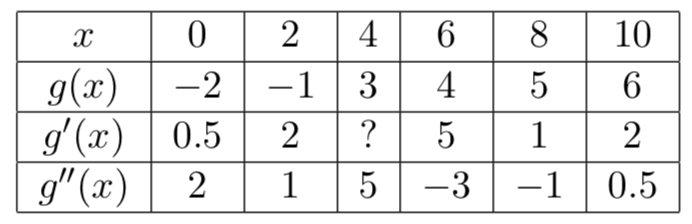
\includegraphics[scale=0.5]{Figures/table1.png}	
	\end{figure}	
	\begin{enumerate}[(a)]
		\item Let $k(x) = g(x)g'(x)$. Find the value of $g'(4)$ if $k'(4)=15$.
		\item Let $r(x) = \frac{\sin(x)}{g(x)}$. Find $r'(0)$.
	\end{enumerate}
        \begin{solution}
          See parts (ii) and (iii) for part (a) in\\ \href{https://dhsp.math.lsa.umich.edu/exams/115exam2/f17/s1.pdf}{https://dhsp.math.lsa.umich.edu/exams/115exam2/f17/s1.pdf}
        \end{solution}
\question Consider the family of functions
\[
f(x) = \frac{ax^b}{e^x}, \quad x \geqslant 0
\]
where $a>0$ and $b>1$ are positive constants. Find the values of $x$ for which the tangent lines of $y = f(x)$ are horizontal. Your answer will contain $a$ and $b$.
\begin{solution}
  We check \[
    f'(x) = \frac{\ddx(ax^b)e^x-ax^b\ddx(e^x)}{(e^x)^2} =
    \frac{abx^{b-1}e^x-ax^be^x}{e^{2x}} = \frac{ax^{b-1}(b-x)}{e^x}
  \]
  So, if we set \(f'(x) = 0\) and observe both \(a>0\) and \(e^x > 0\)
  for all \(x\), we must find all \(x\) such that \(x^{b-1}(b-x) = 0\). Thus,
  the only horizontal tangent lines are at \(x=0\) and \(x=b\).
\end{solution}
\question (Fall 2017 Exam 2) Consider the graph of $h(x)$ below. Note that \(h\) is linear on the intervals $[-4,-1)$, $[-1,1]$ and $[1,2]$, differentiable on $(2, 5)$, and has a sharp corner at $x = 2$.
\begin{center}
  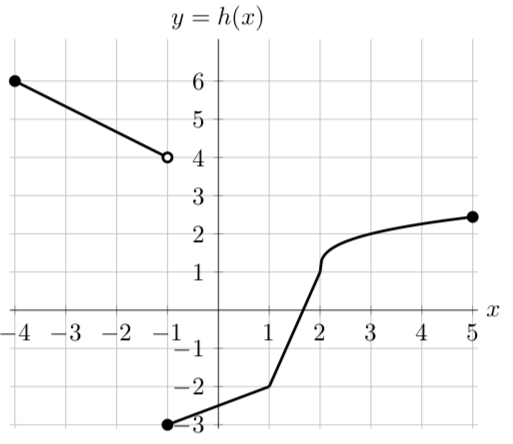
\includegraphics[scale=0.33]{Figures/Exam2Fall2017Problem4}
\end{center}
\vspace{-0.7cm}
Let \(g(x) = xh(x)\). Find \(g'(-2)\).
\begin{solution}
  See part (a)(i) in \href{https://dhsp.math.lsa.umich.edu/exams/115exam2/f17/s4.pdf}{https://dhsp.math.lsa.umich.edu/exams/115exam2/f17/s4.pdf}
\end{solution}
\question The equation of motion for a particle is given by \(s(t) =
  \cos(t) \sin(t) + \sin(t)\). 
  \begin{parts}
  \part Find the velocity and acceleration at time \(t\).
  \part Use \(\sin^2(x)+\cos^2(x) = 1\) to write the velocity
    function \(s'(t)\) in terms of the cosine function. Then factor the result in order to find the exact times when the velocity is \(0\).
  \part Here’s a graph of the position, velocity, and acceleration
    functions together on the same coordinate grid. Circle the letters corresponding to correct statements: \\
    \begin{minipage}{0.45\linewidth}
      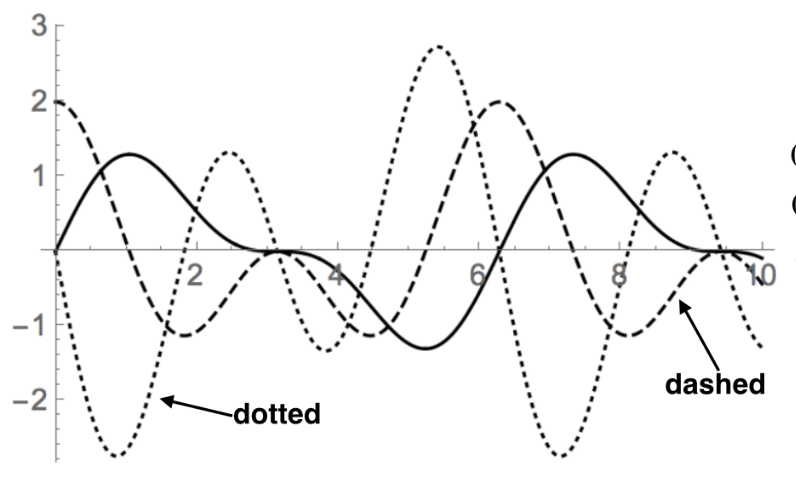
\includegraphics[scale=0.45]{Figures/graphs}
    \end{minipage}
    \begin{minipage}{0.55\linewidth}
      \begin{enumerate}[(a)]
      \item The graph of the position function is dotted.
      \item The graph of the position function is solid.
      \item The graph of the velocity function is dashed.
      \item The graph of the velocity function is dotted.
      \end{enumerate}
    \end{minipage}
  \end{parts}
  \begin{solution}
    \begin{enumerate}[(a)]
    \item The velocity is given by
      \(s'(t) =
      ((\cos(t))^2-(\sin(t))^2)+\cos(t) \).
    \item We rewrite
      \begin{align*}
        v(t) = s'(t) & = ((\cos(t))^2-(\sin(t))^2)+\cos(t)\\
        & =
          ((\cos(t))^2-(1-(\cos(t))^2))+\cos(t)\\
              & = 2(\cos(t))^2+\cos(t)-1\\
        & = (2\cos(t)-1)(\cos(t)+1)
      \end{align*}
      Thus, the velocity is \(0\) whenever \(\cos(t) = -1\) or
      \(\cos(t) = \frac{1}{2}\). This happens at \(t = \pi+k 2\pi\), 
      \(t = \frac{\pi}{3}+k 2\pi\), and \(t = \frac{5\pi}{3}+k 2\pi\)
      for all non-negative integers \(k\).
    \item Statements (b) and (c) are correct. There are a few ways to
      see this.\\
    {\bf Method 1} The velocity function takes value 2 at the origin while the position 
and acceleration take value 0; thus the dashed curve is the velocity
function.  Note also the dashed curve passes through the t axis at 
around 1, approximately \(\pi/3\), and \(\pi\), consistent with the answer to (b). The 
acceleration is the dotted curve—notice the acceleration is negative 
over, say, \((0, \pi/2)\), where  the velocity function (dashed graph) is 
decreasing—where the velocity function has negatively sloped 
tangents.  Thus the solid curve must be the graph of the position 
function.\\
    {\bf Method 2} To identify which curve corresponds to which function, you need not have formulas for position \(s=s(t)\), 
velocity \(v = v(t)\), and acceleration \(a = a(t)\)  For instance, because the dotted curve has negatively sloped 
tangents over, say, \((0, 1/2)\), but neither the dashed curve nor the solid one lies below the t-axis over \((0, 1/2)\), 
the derivative of the function with the dotted graph is not plotted.  Thus the dotted curve corresponds to 
the acceleration function.  Since the dashed curve has negatively sloped tangents over, say, \((0,1)\), the 
derivative of the function with the dashed graph would have a graph lying below the t-axis over \((0, 1)\).   The 
only graph with this property is that of the acceleration.   Thus, the derivative of the function with the 
dashed graph is  the acceleration function.   We conclude that the dashed graph is that  of velocity.  This 
means the solid graph is that of the position function.  
    \end{enumerate}
  \end{solution}
\end{questions}
\end{document}
%%% Local Variables:
%%% mode: latex
%%% TeX-master: t
%%% End:
